\section{Introduction}
% \begin{figure*}[t]
%     \centering
%     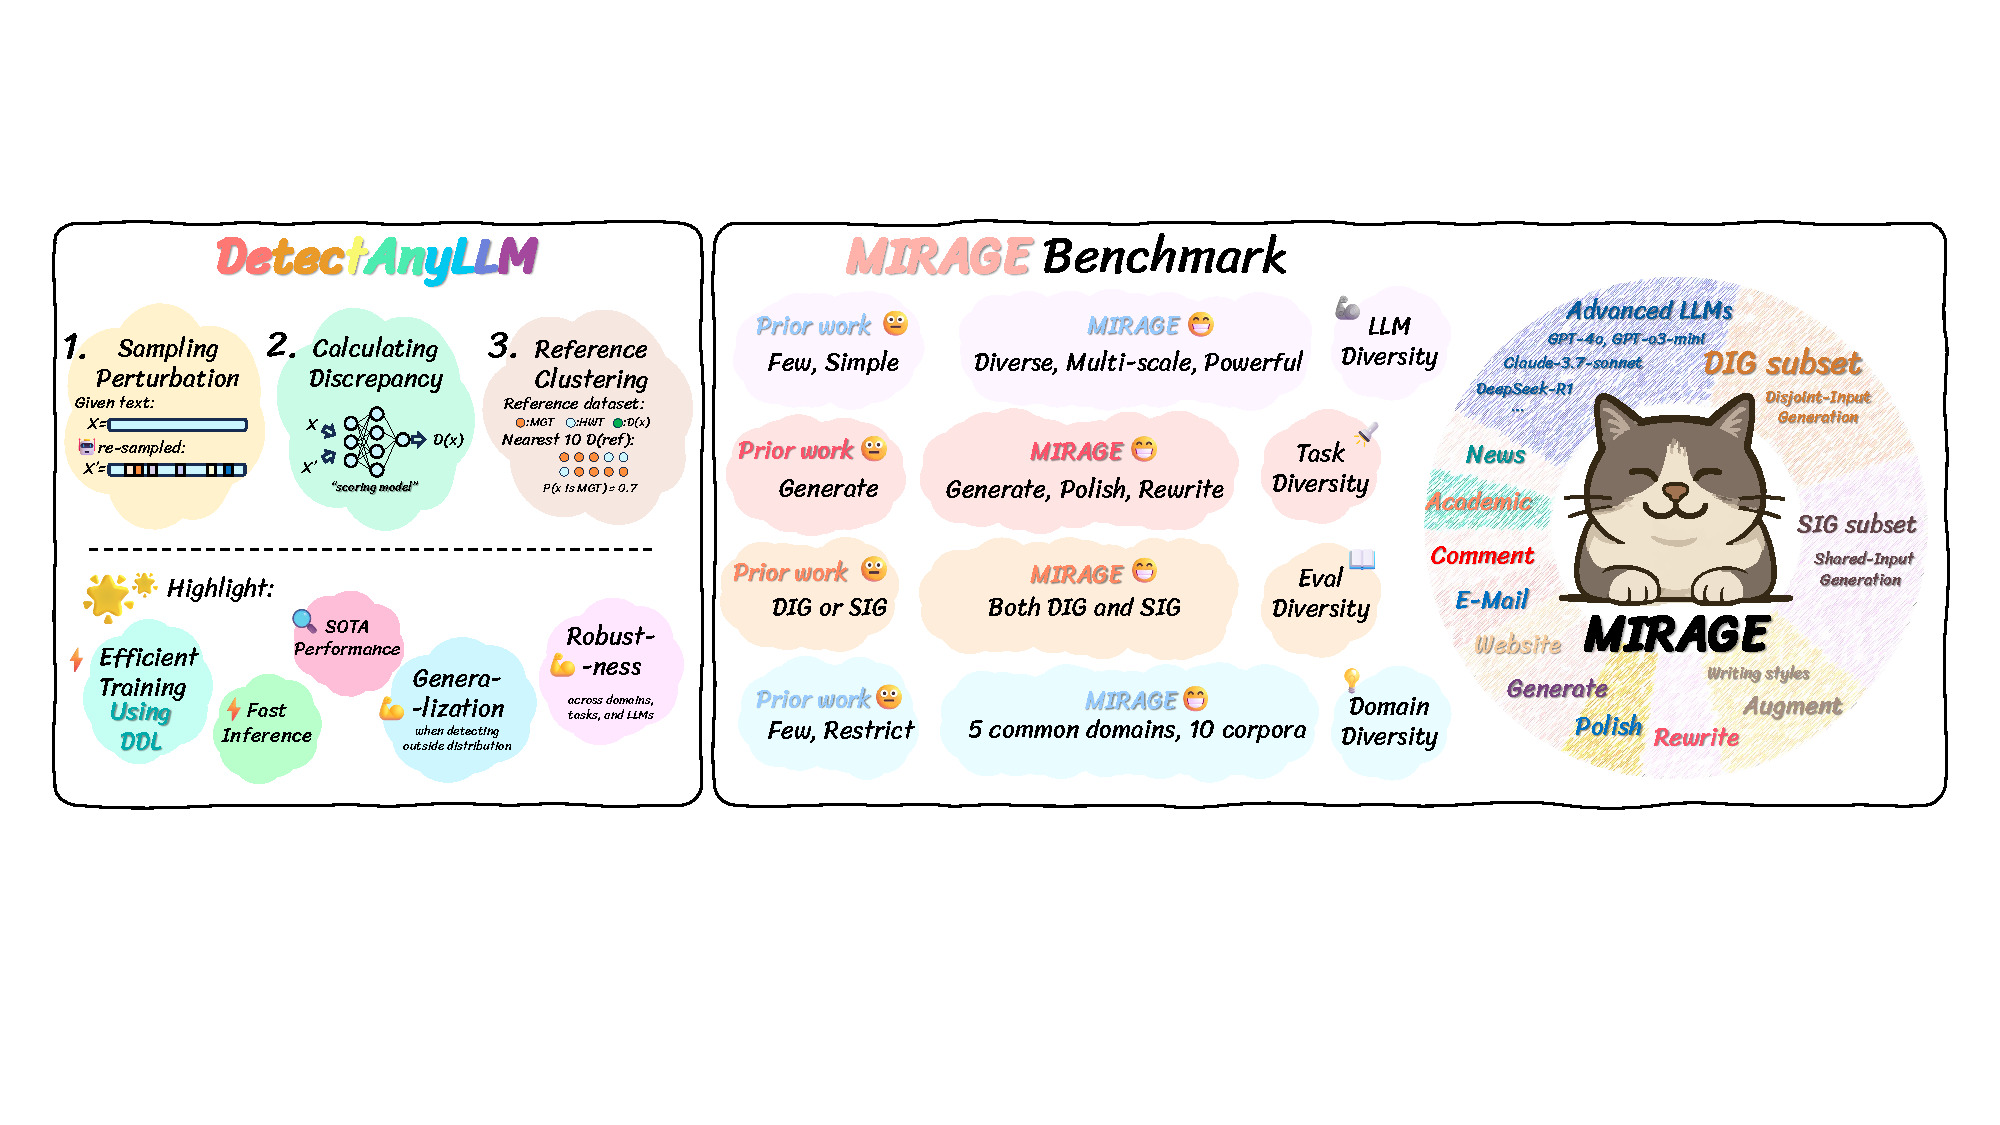
\includegraphics[width=\linewidth]{fig/teaser.pdf}
%     \caption{Overview of our work.}
%     \Description{Simple look of our work.}
%     \label{fig:main}
% \end{figure*}
%\noindent \textbf{Why detect?}
Advanced generative \textit{Large Language Models (LLMs)}~\cite{gpt4, gpt4o, deepseekr1, deepseekv3, gpto1} can easily generate text nearly indistinguishable from human writing~\cite{indistinguish_1, indistinguish_2}.
%
If such technology is misused, it could pose serious risks to society.
%
% For example, 
% in academic research, the inability to distinguish between human-authored papers and LLM-generated content could undermine the credibility of scholarly work. 
%
% Similarly, 
% if we cannot determine whether news reports are written by human journalists or fabricated by LLMs~\cite{fakenews}, the integrity of information and public trust in the media could be significantly compromised. %\lichongyi{this sentence can be removed if we do not have enough space.}
%\noindent \textbf{Task define}
In response to such concern, the task of \textit{Machine-Generated Text Detection (MGTD)} has emerged~\cite{logrank, entropy, likelihood}.
%
MGTD is a binary classification task designed to distinguish whether a given text is completely written by humans or generated (or revised) by a machine.
%
Note that, in this study, MGTD includes detection of both \textit{Machine-Generated Text (MGT)} and \textit{Machine-Revised Text (MRT)}, where MRT refers to text that has been polished or rewritten by a model based on an original \textit{Human-Written Text (HWT)}.


%\noindent \textbf{Baseline? Theory?}
As MGT and MRT have distinct token probability distributions compared to HWT, several MGTD methods have been proposed~\cite{logrank, likelihood, entropy, detectgpt, fastdetectgpt}. 
%
Most of them leverage pre-trained language models, referred to as \textit{scoring models}, to estimate the token probabilities of a given text and compute classification metrics for distinguishing between human-written and machine-generated content.


Existing MGTD methods can be further categorized into zero-shot detection methods~\cite{entropy, lrrandnpr, detectgpt, fastdetectgpt, hart} and training-based detection methods~\cite{logrank, imbd}.
%
%\todel{The performance of zero-shot methods is often constrained, as they rely heavily on the original output distribution of the scoring model~\cite{glimpse}. However, scoring models are usually small-scale LLMs (e.g. GPT-Neo-2.7B~\cite{gpt-neo}), which have limited knowledge and simpler output patterns compared to large-scale models. As a result, they struggle to effectively detect text outside of their original distributions, causing the performance of zero-shot detection to be heavily dependent on the capabilities of the scoring model itself.}
%
Zero-shot methods typically rely on the original output distributions of pre-trained scoring models~\cite{glimpse}, which constrains their performance. This limitation arises because scoring models are often relatively small-scale language models (e.g., GPT-Neo-2.7B~\cite{gpt-neo}), which possess restricted knowledge and comparatively simplistic output patterns. However, detection often happens with texts that deviate from their inherent distribution, making it difficult for these methods to realize reliable detection.
%
Training-based methods use \textit{supervised fine-tuned (SFT)}~\cite{sft, logrank} or \textit{preference learning}~\cite{orpo, dpo, imbd} to align the scoring model's output distribution with that of a specific model.
%
While this approach improves detection performance for that specific model, it often causes the scoring model to overfit the training data~\cite{overfit, outdomain}. As a result, the detector's ability to generalize and remain robust when detecting outside the training distribution is compromised~\cite{fastdetectgpt, survey_necessity_methods_futuredirect, survey_science}. %\lichongyi{why?}

%\noindent \textbf{Motivation}
In this study, we find that the key to improve the generalization and robustness of the detector lies in training the scoring model to capture more intrinsic differences between MGT and HWT, rather than merely optimizing the token probability distributions.
%
Furthermore, we observe that even the most advanced training-based methods~\cite{imbd, pawn} primarily fine-tune the scoring model to align its output distribution with that of the target model they aim to detect, rather than directly training the scoring model as a dedicated detector, which may hinder performance on the MGTD task..

Building on such observations, we propose a novel optimization strategy, \textbf{Direct Discrepancy Learning (DDL)}, that enables the model to \textbf{learn to be a detector rather than another language model} by directly optimizing the scoring model with its output classification metric.
%
DDL aims to free the scoring model from the constraints of its original language model identity so that it can focus on learning the intrinsic knowledge of MGT detection rather than merely fitting the distribution of the training data. 

Furthermore, as the fusion of prior approaches~\cite{fastdetectgpt, imbd} and DDL, we propose \textbf{DetectAnyLLM}, a unified MGTD framework.
%
DetectAnyLLM achieves efficient and robust detection through three steps comprising \textit{re-sampling}, \textit{discrepancy calculation}, and \textit{reference clustering}.
%
Such a framework distills the core insights of existing methods~\cite{detectgpt, fastdetectgpt} while leveraging DDL to enhance the model’s generalization capabilities and improve detection robustness.
%\lichongyi{we need a figure to show the performance improvement of our strategy. We can put it on the top right of the first page.}
\begin{table*}[htbp]
    \centering
    \caption{Comparison between MIRAGE and existing MGTD benchmark datasets. ``Size" is the capacity of the test set. ``SIG" denotes Shared-Input Generation and ``DIG" denotes Disjoint-Input Generation. ``Commercial" refers to the use of frontier proprietary LLMs (e.g., GPT-4o). MIRAGE is the most diverse benchmark in terms of domain, tasks, and source LLMs. MIRAGE leverages powerful commercial LLMs to generate and revise text, increasing the difficulty of detection and the realism of evaluation, enabling a more faithful evaluation of detector robustness. Furthermore, MIRAGE introduces a novel dual-scenario evaluation strategy —DIG and SIG— allowing more comprehensive assessment of both accuracy and generalization capacity.}
    \renewcommand{\arraystretch}{1.25}
    \resizebox{\linewidth}{!}{
    \begin{tabular}{l|ccc|c|ccc|ccc}
    \hline

    \hline

    \hline
    &\multicolumn{3}{c|}{\textbf{Data Statistic}}&\multicolumn{1}{c|}{\textbf{LLMs}}&\multicolumn{3}{c|}{\textbf{MGT Tasks}}&\multicolumn{3}{c}{\textbf{Other}}\\
    \textbf{Benchmark}& Size & Domain Coverage & Corpus & Commercial & Generate & Polish & Rewrite & Aug. & SIG & DIG\\
    \hline
    TuringBench~\cite{turingbench}& 40K & News & 3 & \wrong & \correct & \wrong & \wrong & \wrong & \wrong & \correct\\
    HC3~\cite{hc3}& 85K & QA/Comment/Academic & 5 & 1  & \correct & \wrong & \wrong & \wrong & - & - \\
    M4~\cite{m4bench}& 24.5K & QA/Comment/Academic/News & 11 & 2 & \correct & \wrong & \wrong & \correct & \correct & \wrong\\
    MAGE~\cite{mage}& 29K & QA/Comment/News/Academic/Story & 10 & 3 & \correct & \wrong & \wrong & \correct & \correct & \wrong \\
    RAID~\cite{raid}& 628.7K & News/Academic/Comment/Literature& 11& 3 & \correct & \wrong & \correct & \correct & \correct & \wrong\\
    DetectRL~\cite{detectrl}&134.4K& Academic/Comment & 4 & 2&\correct&\wrong&\correct&\correct&\correct&\wrong \\
    HART~\cite{hart}&16K& News/Literature/Academic& 4 & 4 & \correct & \correct &\correct &\correct & \wrong & \correct \\    
    \rowcolor[HTML]{fff5f4}
    \textbf{MIRAGE (ours)}&93.8K &Academic/Comment/Email/News/Website & 10 & 13 & \correct & \correct & \correct & \correct & \correct & \correct \\
    \hline

    \hline

    \hline
    \end{tabular}
    }
    \label{tab:benchmarks}
\end{table*}

\begin{figure}[t]
    \centering
    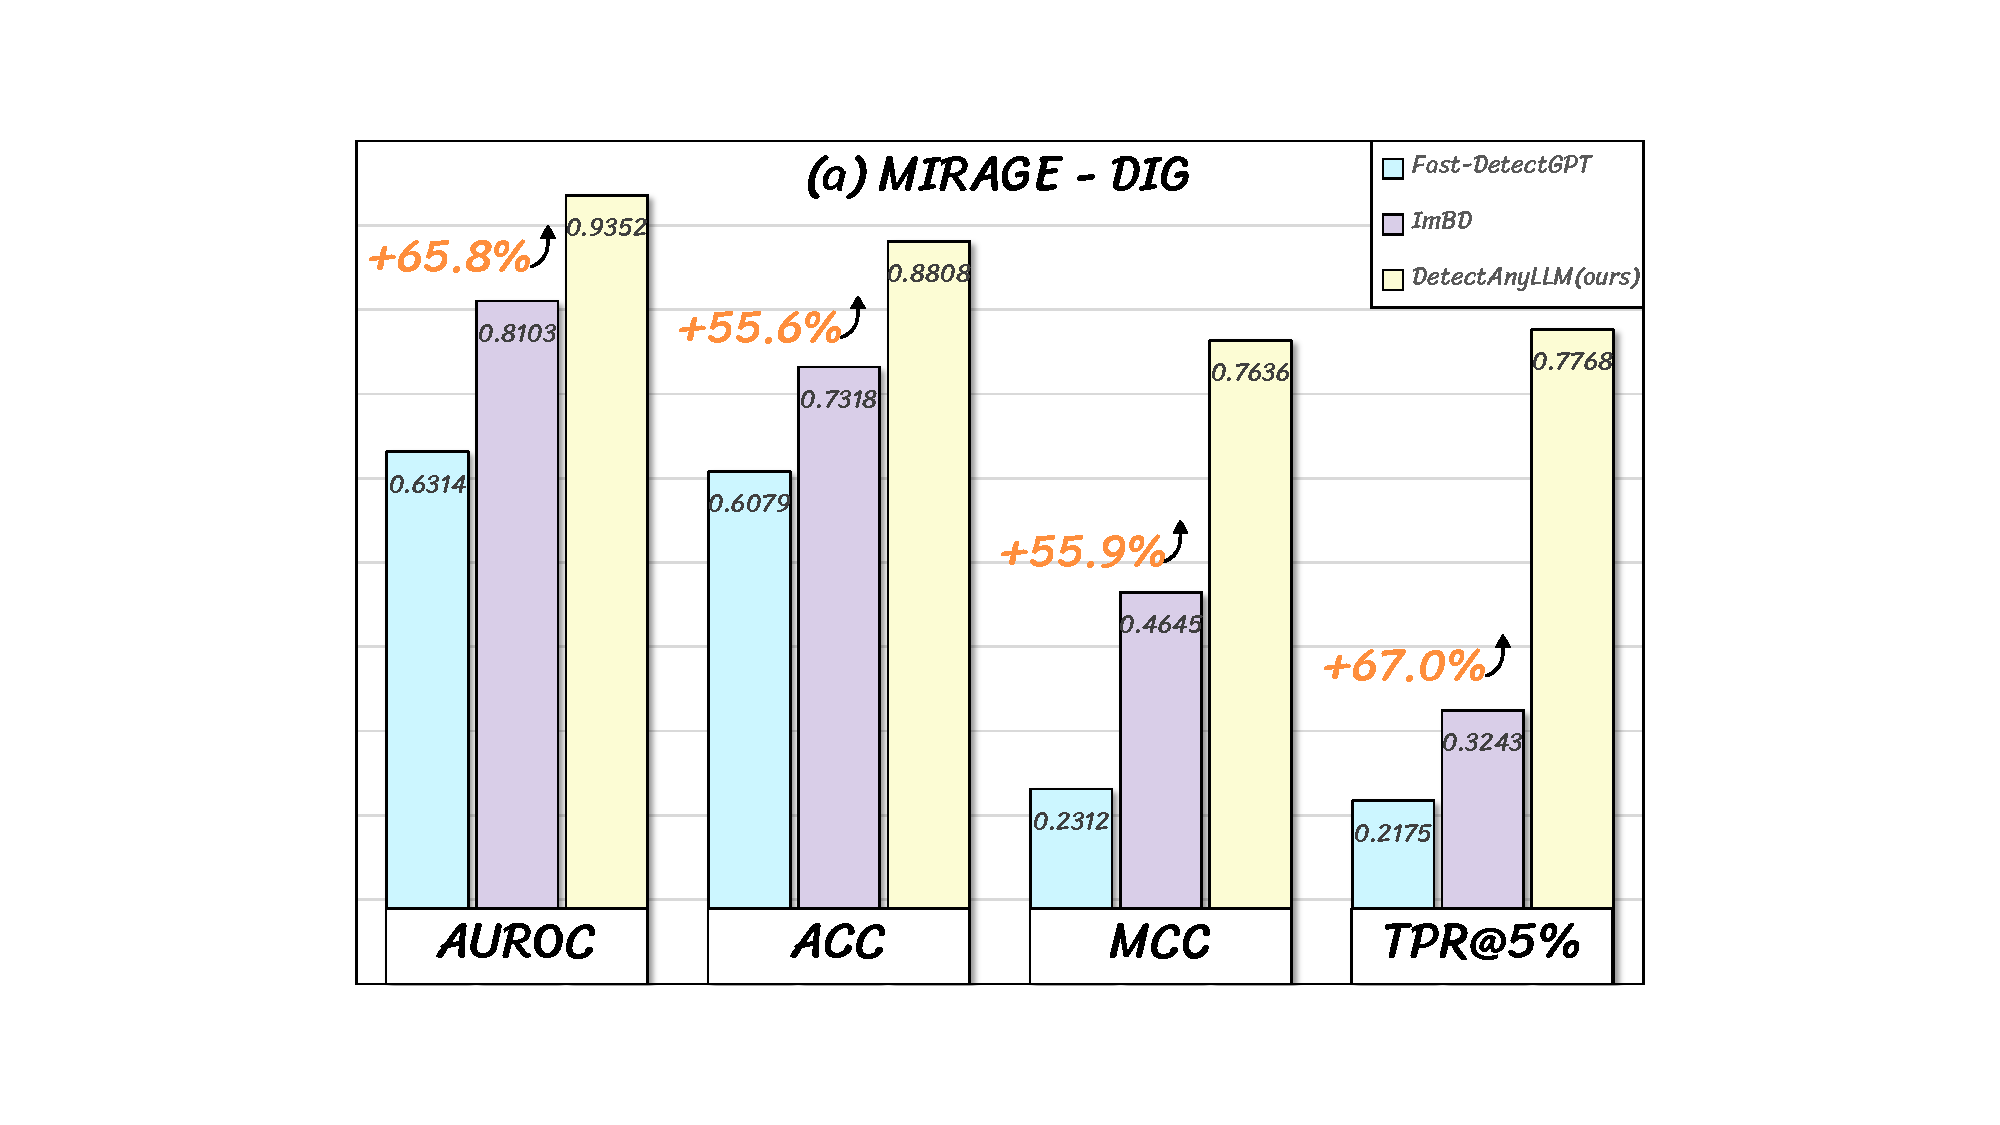
\includegraphics[width=0.985\linewidth]{fig/performance_comparison.pdf}
    \caption{Performance on MIRAGE-DIG for DetectAnyLLM and state-of-the-art methods, including Fast-DetectGPT~\cite{fastdetectgpt} and ImBD~\cite{imbd}. Improvement: $(new-old)/(1.0-old)$.}
    \Description{Performance Comparison on MIRAGE. The DIG subset reflects abilities across domains, and the SIG subset reflects abilities across generators.}
    \label{fig:performance_comparison}
\end{figure}

%\noindent \textbf{Benchmark}
In addition, despite the emergence of various MGTD studies, there remains a lack of comprehensive benchmarks~\cite{survey_necessity_methods_futuredirect}.
%
Existing benchmarks~\cite{mage, mgtbench, detectrl} suffer from several significant deficiencies: \textbf{1) Limited focus on MRT:} Most benchmark datasets, such as MGTBench~\cite{mgtbench}, focus solely on MGT while neglecting the detection of MRT. \textbf{2) Narrow range of source LLMs:} Most benchmarks rely on small-scale, open-source models, whereas real-world applications often involve advanced, closed-source LLMs such as GPT-4o~\cite{gpt4o} and DeepSeek-R1~\cite{deepseekr1}.  \textbf{3) Restricted domain coverage:} Benchmarks such as HC3~\cite{hc3} typically sample text from only one or a few domains, neglecting the domain sensitivity of machine-generated text.
%
These deficiencies highlight a significant gap between existing benchmark datasets and real-world applications, indicating that current benchmarks fail to comprehensively and objectively reflect real-world detection challenges.


Although some recent studies~\cite{survey_necessity_methods_futuredirect, hart} have recognized this issue, their datasets remain insufficiently comprehensive.
%
To facilitate further research,  we construct \textbf{MIRAGE}, the largest multi-task MGTD benchmark that provides the richest variety of commercial LLMs and the most comprehensive text domains in MGTD research.
%
As shown in ~\Cref{tab:benchmarks}, MIRAGE samples text from \textbf{10 corpora} in \textbf{5 common domains}, and uses \textbf{17 advanced mainstream LLMs} for text generation or revision, creating over \textbf{93K HWT-MGT pairs}.
%
MIRAGE establishes a more realistic and reliable evaluation standard, bridging the gap between research and real-world applications.


Though existing detection methods have demonstrated seemingly outstanding performance (AUC > 0.9) on previous benchmarks~\cite{imbd, detectrl}, they exhibit significant weaknesses when evaluated on MIRAGE, as ~\Cref{fig:performance_comparison} shown.
%
This reveals the generalization and robustness of prior methods require substantial improvement. 
%
In contrast, DetectAnyLLM still performs well, achieving an average of \red{0.9352} AUROC and \red{0.7636} MCC on the MIRAGE-DIG subset.
%
Such performance powerfully demonstrates the effectness and superior generalization of DDL.


Our contributions can be summarized into the following points:


\begin{itemize}[leftmargin=*]
    \item We propose a novel optimization strategy for MGTD, termed \textbf{Direct Discrepancy Learning (DDL)}, enabling the model to
    %function explicitly as a detector rather than another language model, thereby 
    directly acquire task-oriented knowledge. DDL greatly improve detector's generalization and robustness with fewer computational resources and no additional training data.
    \item We construct a comprehensive benchmark dataset for MGTD, named \textbf{MIRAGE}, which covers the most diverse text domains, MGT tasks, and source LLMs. MIRAGE novelly focuses on using commercial LLMs to generate data, enhancing the realism and practical relevance of evaluation.
    %Extensive experiments on MIRAGE reveal that existing MGTD methods heavily fall short in performance across various challenging scenarios.
    \item We present \textbf{DetectAnyLLM} framework, unifying prior works and DDL. DetectAnyLLM achieve \textbf{50\%-70\%} performance improvement over previous state-of-the-art methods, realizing a generalizable and robust detection across domains and models.
    %—demonstrating the effectiveness and efficiency of DDL.
\end{itemize}

% \noindent \textbf{Contribution}